\documentclass[12pt, a4paper]{article}
\usepackage[a4paper, left=2cm, right=2cm, top=3cm, bottom=3cm]{geometry}

\usepackage[english]{babel}
\usepackage[utf8]{inputenc}
\usepackage{fancyhdr}

\usepackage{enumitem}
\usepackage{amsmath}
\usepackage{mathtools}

\usepackage{tikz}
\usetikzlibrary{arrows.meta,shapes.multipart}

\pagestyle{fancy}
\fancyhf{}
\lhead{Simon Scherello, XXXXXX}
\chead{Blatt 02}
\rhead{Til Mohr, 405959}

\begin{document}

\section*{Aufgabe 7}
\begin{enumerate}[label=\alph*)]
	\item Knoten beinhalten Namen über dem Grad.\\
		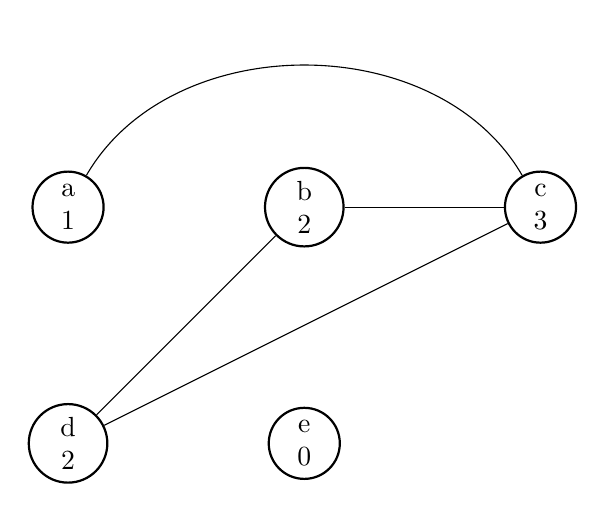
\begin{tikzpicture}[every node/.style={circle,thick,draw,align=center}, node distance=3cm]
			\node (a) {a\\1};
			\node[right of=a] (b) {b\\2};
			\node[right of=b] (c) {c\\3};
			\node[below of=a] (d) {d\\2};
			\node[right of=d] (e) {e\\0};
			
			\path (a) edge[bend left=60] (c);
			\path (b) edge (c);
			\path (b) edge (d);
			\path (c) edge (d);
		\end{tikzpicture}
	
	\item Knoten beinhalten Namen über [Innengrad, Außengrad].\\
		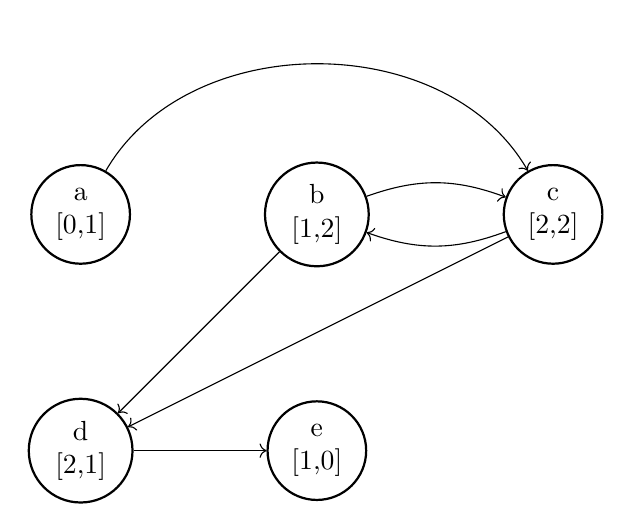
\begin{tikzpicture}[every node/.style={circle,thick,draw,align=center}, node distance=3cm]
			\node (a) {a\\{[0,1]}};
			\node[right of=a] (b) {b\\{[1,2]}};
			\node[right of=b] (c) {c\\{[2,2]}};
			\node[below of=a] (d) {d\\{[2,1]}};
			\node[right of=d] (e) {e\\{[1,0]}};
			
			\path[->] (a) edge[bend left=60] (c);
			\path[->] (b) edge[bend left=20] (c);
			\path[->] (b) edge (d);
			\path[->] (c) edge[bend left=20] (b);
			\path[->] (c) edge (d);
			\path[->] (d) edge (e);
		\end{tikzpicture}
	
	\item Nein, $G_1$ ist nicht dem $G_2$ zugrundeliegende ungerichtete Graph. Wäre dies nämlich der Fall, so dürfe es in $G_2$ keine Kante $(d,e)$ geben.
\end{enumerate}



\newpage



\section*{Aufgabe 8}
\begin{enumerate}[label=\alph*)]
	\item $V=\{a,b,c,d,e,f,g,h,k\}$\\
		$E=\{\{a,d\},\{b,c\},\{b,d\},\{b,e\},\{b,f\},\{c,e\},\{d,e\},\{d,g\},\{e,f\},\{e,g\},\{e,k\},\{f,h\},\{f,k\},\{h,k\}\}$
	
	\item $W=(a,d,b,c,e,b,f,h)$
	
	\item Nein, es ist unmöglich, dass ein Weg elementar, aber nicht einfach ist.\\
		Jeder Weg $W$ in einem Graphen $G=(V,E)$, der nicht einfach ist, besitzt ja mindestens eine Kantenwiederholung an einer Kante $(i,j) \in E$ mit $i,j \in V$. Aus diesem Grund muss $W$ auch die Kanten $i,j$ mind. zweimal durchlaufen. Also gibt es auch eine Knotenwiederholung an $i,j$, weshalb $W$ nicht elementar sein kann.
		
	\item $W=(a,d,e,k)$
	
	\item $W=(a,d,g,e,b,d,e,c,b,f,e,k,h,f,k)$
\end{enumerate}



\newpage



\section*{Aufgabe 9}
\begin{enumerate}[label=\alph*)]
	\item Ungerichteter Graph:\\
		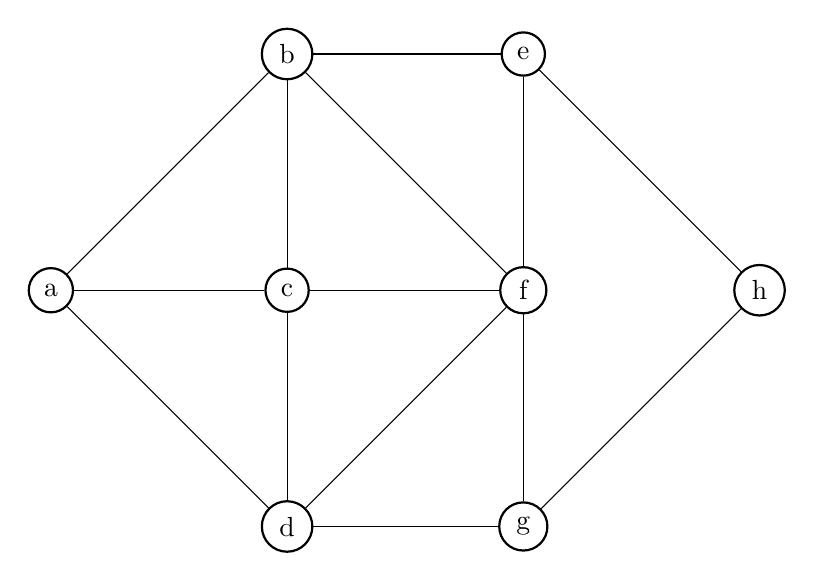
\begin{tikzpicture}[every node/.style={circle,thick,draw,align=center}, node distance=3cm]
			\node (a) {a};
			\node[right of=a] (c) {c};
			\node[above of=c] (b) {b};
			\node[below of=c] (d) {d};
			\node[right of=b] (e) {e};
			\node[right of=c] (f) {f};
			\node[right of=d] (g) {g};
			\node[right of=f] (h) {h};
			
			\path (a) edge (b);
			\path (a) edge (c);
			\path (a) edge (d);
			\path (b) edge (e);
			\path (b) edge (c);
			\path (b) edge (f);
			\path (c) edge (d);
			\path (c) edge (f);
			\path (d) edge (f);
			\path (d) edge (g);
			\path (e) edge (f);
			\path (e) edge (h);
			\path (f) edge (g);
			\path (g) edge (h);
		\end{tikzpicture}

	\item Der Graph ist zusammenhängend, da es in dem ungerichteten Graphen von jedem Knoten möglich ist, jeden anderen zu erreichen.\\
		Der Graph ist nicht stark zusammenhängend, da es in dem gerichteten Graphen nicht möglich ist, von jedem Knoten jeden anderen zu erreichen. Beispielsweise kann $h$ nicht $e$ erreichen.
		
	\item
		\begin{enumerate}[label=(\roman*)]
			\item $\delta(X_1)=\{\{a,d\},\{c,d\},\{b,f\},\{c,f\},\{e,f\},\{e,h\}\}$\\
				$\delta^+(X_1)=\{(c,d),(c,f),(e,f),(e,h)\}$\\
				$\delta^-(X_1)=\{(d,a),(f,b),(f,c),(f,e)\}$
			
			\item $\delta(X_2)=\{\{b,a\},\{b,c\},\{b,f\},\{e,f\},\{h,g\}\}$\\
				$\delta^+(X_2)=\{(a,b),(c,b),(f,b),(f,e),(g,h)\}$\\
				$\delta^-(X_2)=\{(e,f)\}$
		\end{enumerate}
	
	\item
		\begin{enumerate}[label=(\roman*)]
			\item $Y_1$ bildet keinen Schnitt. Denn in $Y_1$ sind die Kanten $\{b,e\}$ und $\{b,f\}$ enthalten. Folglich müsste in der zugehörigen Knotenmenge $X$ entweder $b$ ODER $e$ und $f$ enthalten sein.\\
				\\Angenommen $b \in X$. Da $\{b,e\} \not\in Y_1$ müsste $c \in X$ gelten. Dann müsste aber auch $\{c,f\} \in Y_1$. \textbf{Geht nicht.}\\
				Angenommen $e,f \in X$. Da $\{f,c\} \not\in Y_1$ müsste $c \in X$ gelten. Dann müsste aber auch $\{c,b\} \in Y_1$. \textbf{Geht nicht.}\\
				\\Daher bildet $Y_1$ keinen Schnitt.
			
			\item $Y_2 = \delta(\{a,h\})$
		\end{enumerate}
	
	\item Es gibt keinen gerichteten Schnitt, welcher $f$ von $c$ trennt. Um $f$ von $c$ zu trennen, müsste entweder $f$ oder $c$ in der Knotenmenge $X$ des Schnittes liegen. Jedoch wäre dann weder $\delta^+(X)$ noch $\delta^-(X)$ leer, da sowohl $(c,f)$ als auch $(f,c)$ in unserem Graphen existiert. Damit gibt es keinen solchen gerichteten Schnitt.
\end{enumerate}



\newpage



\section*{Aufgabe 10}
\begin{enumerate}[label=\alph*)]
	\item Wir modellieren das Problem als Knotenfärbungsproblem in einem ungerichteten Graphen $G=(V,E)$ mit:
		\begin{itemize}
			\item $V \coloneqq $Länder
			\item $E \coloneqq \{\{i,j\} \vert i,j \in V, i \neq j, \text{i und j haben eine gemeinsame Grenze}\}$
			\item $C \coloneqq $Farbauswahl
		\end{itemize}
		Eine zulässige $\vert C \vert$-Färbung von $G$ entspricht einer Zuordnung von Farben zu den Ländern auf der Landkarte, sodass keine benachbarten Länder dieselbe Farbe besitzen.\\
		Somit existiert eine zulässige Zuordnung der Farben zu den Ländern auf der Landkarte genau dann, wenn der Graph $G$ $\vert C \vert$-färbbar ist.
	
	\item Betrachtet man sich die Gegend DE-FR-BEL-LUX, so wird es schnell klar, dass man mind. 4 Farben benötigt:\\
		Färbt man DE rot, kann man FR blau färben. BEL nun grün. Nun könnten wir LUX keine der drei Farben rot, blau, grün zuuordnen, da die Landkarte sonst zwei benachbarte Länder mit derselben Färbung hätte.\\
		Also benötigen wir mind. 4 Farben.
	
	\item Färbung mit 4 Farben:\\
		\begin{center}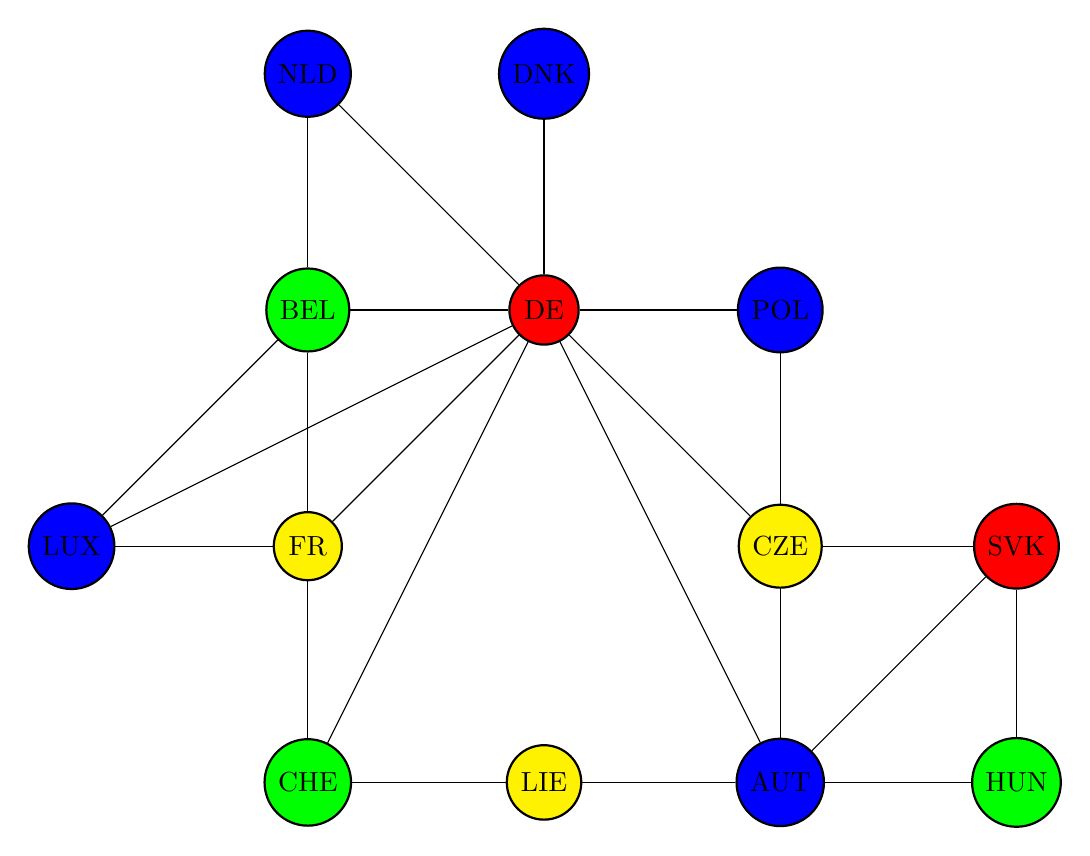
\begin{tikzpicture}[every node/.style={circle,thick,draw,align=center}, node distance=3cm]
			\node[fill=red] (DE) {DE};
			\node[fill=blue, above of=DE] (DNK) {DNK};
			\node[fill=blue, left of=DNK] (NLD) {NLD};
			\node[fill=green, left of=DE] (BEL) {BEL};
			\node[fill=yellow, below of=BEL] (FR) {FR};
			\node[fill=blue, left of=FR] (LUX) {LUX};
			\node[fill=green, below of=FR] (CHE) {CHE};
			\node[fill=yellow, right of=CHE] (LIE) {LIE};
			\node[fill=blue, right of=LIE] (AUT) {AUT};
			\node[fill=yellow, above of=AUT] (CZE) {CZE};
			\node[fill=blue, right of=DE] (POL) {POL};
			\node[fill=red, right of=CZE] (SVK) {SVK};
			\node[fill=green, right of=AUT] (HUN) {HUN};
			
			\path (DE) edge (DNK);
			\path (DE) edge (NLD);
			\path (DE) edge (BEL);
			\path (NLD) edge (BEL);
			\path (DE) edge (LUX);
			\path (BEL) edge (LUX);
			\path (DE) edge (FR);
			\path (FR) edge (LUX);
			\path (FR) edge (BEL);
			\path (DE) edge (CHE);
			\path (FR) edge (CHE);
			\path (CHE) edge (LIE);
			\path (DE) edge (AUT);
			\path (LIE) edge (AUT);
			\path (AUT) edge (CZE);
			\path (DE) edge (CZE);
			\path (POL) edge (CZE);
			\path (DE) edge (POL);
			\path (CZE) edge (SVK);
			\path (AUT) edge (SVK);
			\path (AUT) edge (HUN);
			\path (SVK) edge (HUN);
		\end{tikzpicture}\end{center}
\end{enumerate}



\newpage



\section*{Aufgabe 11}
Wir modellieren das Problem als Knotenfärbungsproblem in einem ungerichteten Graphen $G=(V,E)$ mit:
\begin{itemize}
	\item $V \coloneqq $Sendestationen
	\item $E \coloneqq \{\{i,j\} \vert i,j \in V, i \neq j, \text{Sendebereiche von i und j überschneiden sich}\}$
	\item $C \coloneqq \{\text{1758.02 MHz, 1768.02 MHz, 1780.02 MHz}\}$
\end{itemize}
Eine zulässige $3$-Färbung von $G$ entspricht einer Zuordnung von Frequenzen zu den Sendestationen, sodass keine Inteferenz oder ein sonstiger Nachteil entsteht.\\
Somit existiert eine zulässige Zuordnung der Frequenzen zu den Sendestationen genau dann, wenn der Graph $G$ $3$-färbbar ist.\\

Betrachtet man das Beispiel aus der Aufgabenstellung, so bekommen wir folgenden Graphen, den wir auch färben können.
Hierbei strahlt eine rot gefärbte Sendestation auf der Frequenz 1758.02 MHz aus, eine grün gefärbte auf der Frequenz 1768.02 MHz und eine blau gefärbte auf der Frequenz 1780.02 MHz.\\
\begin{center}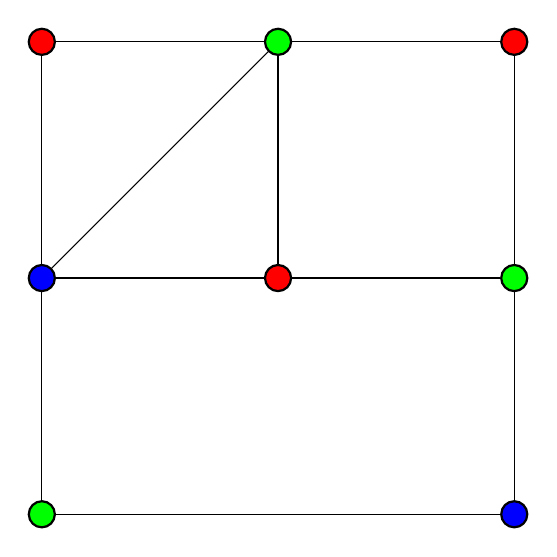
\begin{tikzpicture}[every node/.style={circle,thick,draw,align=center}, node distance=3cm]
	\node[fill=red] (a) {};
	\node[fill=green, right of=a] (b) {};
	\node[fill=red, right of=b] (c) {};
	\node[fill=blue, below of=a] (d) {};
	\node[fill=red, right of=d] (e) {};
	\node[fill=green, right of=e] (f) {};
	\node[fill=green, below of=d] (g) {};
	\node[fill=blue, below of=f] (h) {};
	
	\path (a) edge (b);
	\path (b) edge (c);
	\path (a) edge (d);
	\path (b) edge (d);
	\path (b) edge (e);
	\path (c) edge (f);
	\path (d) edge (e);
	\path (e) edge (f);
	\path (d) edge (g);
	\path (f) edge (h);
	\path (g) edge (h);
\end{tikzpicture}\end{center}



\newpage



\section*{Aufgabe 12}
Die $K$ Müllwägen können reduziert werden auf $1$ Müllwagen, da, immer wenn einer der $K$ Müllwägen von seiner Route in das Depot zurückkehrt, kann derselbe Müllwagen die Route des ursprünglich nächsten Müllwagens übernehmen.\\
Also können wir das Problem auf $1$ Müllwagen reduzieren.\\

Nun modellieren wir das Problem als Eulerkreis in dem ungerichteten Straßennetzt $G$.\\
Eine zulässiger Eulerkreis in $G$ entspricht einer korrekten Route von dem $1$ Müllwagen durch das Aachener Straßennetz, wobei nur jede Straße einmal besucht wird.\\
Somit existiert eine zulässige Route durch das Straßennetzt genau dann, wenn der Graph $G$ einen Eulerkreis besitzt.


\newpage



\section*{Aufgabe 13}
Wir modellieren das Problem als Knotenfärbungsproblem in einem ungerichteten Graphen $G=(V,E)$ mit:
\begin{itemize}
	\item $V \coloneqq \{11, 12, 13, 14, 21, 22, 23, 24, 31, 32, 33, 34, 41, 42, 43, 44\}$
	\item $E \coloneqq \{\{i,j\} \vert i,j \in V, i \neq j, \text{i und j sind in derselben Spalte / Zeile / 2x2-Kästchen}\}$
	\item $C \coloneqq \{1,2,3,4\}$
\end{itemize}
Jeder Knoten in $V$ ist hierbei ein Feld aus dem 4x4-Sudoku.\\
Eine Kante wird genau dann eingeführt, wenn es eine Sudoko-Abhängigkeit zwischen zwei Knoten gibt. Dies ist genau dann der Fall, wenn beide Knoten entweder im selben 2x2-Kästchen sind oder in derselben Spalte / Zeile.\\
Unsere Farben sind hier die 4 Zahlen, die zur Auswahl für jedes Feld stehen.\\

Eine zulässige $4$-Färbung von $G$ entspricht einer korrekten Zuweisung der Zahlen zu den Feldern, also eine Lösung des 4x4-Sudokus..\\
Somit existiert eine zulässige Lösung des 4x4-Sudokus genau dann, wenn der Graph $G$ $4$-färbbar ist.\\

Um die Ausgangsposition des Sudokus in den Graphen zu übertragen, muss man lediglich die betroffenen Felder im Voraus färben, anschließend kann man versuchen das Knotenfärbungsproblem zu lösen.



\end{document}